\documentclass[a4paper,10pt]{article}
\usepackage{%
	amsmath,%
	amsfonts,%
	amssymb,%
	amsthm,%
	hyperref,%
	url,%
	latexsym,%
	epsfig,%
	graphicx,%
	psfrag,%
	subfigure,%	
	color,%
	tikz,%
	pgf,%
	pgfplots,%
	pgfplotstable,%
	pgfpages%
}

\usepgflibrary{shapes}
\usetikzlibrary{%
  arrows,%
	backgrounds,%
	chains,%
	decorations.pathmorphing,% /pgf/decoration/random steps | erste Graphik
	decorations.text,%
	matrix,%
  positioning,% wg. " of "
  fit,%
	patterns,%
  petri,%
	plotmarks,%
  scopes,%
	shadows,%
  shapes.misc,% wg. rounded rectangle
  shapes.arrows,%
	shapes.callouts,%
  shapes%
}

\newcommand{\beq}{\begin{equation}}
\newcommand{\eeq}{\end{equation}}
\newcommand{\beqn}{\[}
\newcommand{\eeqn}{\]}
\newcommand{\bea}{\begin{eqnarray}}
\newcommand{\eea}{\end{eqnarray}}
\newcommand{\bean}{\begin{eqnarray*}}
\newcommand{\eean}{\end{eqnarray*}}
\newcommand{\re}{\mbox{$\mathfrak{Re}$}}
\newcommand{\bit}{\begin{itemize}}
\newcommand{\eit}{\end{itemize}}
\newcommand{\ben}{\begin{enumerate}}
\newcommand{\een}{\end{enumerate}}

\theoremstyle{plain}
\newtheorem{thm}{Theorem}[section]
\newtheorem{lem}[thm]{Lemma}
\newtheorem{prop}[thm]{Proposition}
\newtheorem{cor}[thm]{Corollary}

\theoremstyle{definition}
\newtheorem{defn}[thm]{Definition}
\newtheorem{conj}[thm]{Conjecture}
\newtheorem{exmp}[thm]{Example}

%\theoremstyle{remark}
\newtheorem{rem}{Remark}
\newtheorem{note}{Note}

\date{}
\title{Lecture 1: The Poisson Process}
\author{Parimal Parag}

\begin{document}
\maketitle

\section{The Poisson Process}
Let \noindent $(\Omega, \mathcal{F}, \mathcal{P})$ be a probability space.
\begin{defn}[Point Process] A stochastic process $\{N_{t}, t\geqslant 0\}$ is a \textbf{point process} if
\begin{enumerate}
  \item $N_{0} = 0$.
  \item $t\mapsto N_{t} (\omega)$ is non-decreasing, integer valued, right continuous and at points of discontinuity (wherever it has jumps) $(N_{t}- N_{t^{-}})\leqslant 1, \hspace{0.1cm} \forall \quad \omega \in \Omega$. 
\end{enumerate}
\end{defn} 
\begin{defn}[Simple Point Process] A \textbf{simple point process} is a point process of jump size 1.
\end{defn}

\begin{defn}[Stationary Increment Point Process] Let $0\leq t_{1}<t_{2}...,<t_{n}$. If $(N_{t_{n}}-N_{t_{n-1}},N_{t_{n-1}}-N_{t_{n-2}},...,N_{t_{1}})$ has the same joint distribution as $(N_{t_{n}+t}-N_{t_{n-1}+t},...,N_{t_{1}+t}), ~ \forall t \geqslant 0$, $\{N_{t}, t\geqslant 0\}$ is called \textbf{stationary increment point process}.
\end{defn}
\begin{defn}[Stationary Independent Increment Point Process]  We call it to be \textbf{stationary independent increment process} if these random variables are also independent of each other.
\end{defn}

\begin{figure}[hhhh]
\center
	\begin{tikzpicture}
[node distance=1cm, draw=black, thick, >=stealth',
axes/.style=,
codeword/.style={rectangle, draw=black, inner sep=0pt, minimum height=0.8cm, minimum width=0.5cm}]

\begin{scope}[axes]
\draw[->] (0,0) -- (8,0) node[right] {$t$} coordinate (time);
\draw[->] (0,0) -- (0,5) node[above] {$N(t)$} coordinate (number of  events);
\foreach \x/\xtext in {1/S_1, 2/S_2, 5/S_3,7/S_4}
	\draw[xshift=\x cm] (0pt,1pt) -- (0pt,-1pt) node[below,fill=white] {$\xtext$};
\foreach \y/\ytext in {1,...,4}
	\draw[yshift=\y cm] (1pt,0pt) -- (-1pt,0pt) node[left,fill=white] {$\ytext$};
\end{scope}
\draw[] (0,0)--(1,0)--(1,1)--(2,1)--(2,2)--(5,2)--(5,3)--(7,3)--(7,4)--(8,4);
\end{tikzpicture}

 % \caption{}\label{}
\end{figure}
\noindent The points of discontinuity corresponds to the arrival instants of the point process. Let $X_{n}$  denote the inter arrival time between $(n-1)^{th}$ and $n^{th}$ arrival. Further, let, $S_{0}=0,~ S_{n}= \sum^{n}_{k=1}X_{k}$. $S_{n}$ is the arrival instant of of $n^{th}$ point. The arrival at time zero is not counted.

\begin{defn}[Poisson Process]
The point process $\{N_{t},~ t\geq0\} $ is called a \textbf{Poisson process} with rate $\lambda$, if $\{X_{n},~n\geq 1\}$ is an $iid$ $exp(\lambda)$ process, $ 0<\lambda<\infty$.  i.e.
 \begin{equation*}
  P(X_{1}\leq x) = 
	\begin{cases}
		1-e^{-\lambda x}, & x\geq 0   \\
		0,  & \text{ else}.
	\end{cases}
\end{equation*}
\end{defn}

\textbf{Remarks:} Observe that 
\begin{align*}
\{S_{n}\leq t\} &=  \{N_{t}\geq n \},\\
\{S_{n}\leq t, S_{n+1}> t \} &= \{N_{t}= n\},\quad\mathrm{and} \\
\Pr\{X_{n} = 0\} &= \Pr\{X_n\leq 0\} = 0.
\end{align*}
Also, by Strong Law of Large Numbers (SLLN), 
\begin{equation*}
\lim_{n \to \infty} \frac{S_{n}}{n} = E[X_{1}] = \frac{1}{\lambda}\quad\mathrm{a.s.} 
\end{equation*}
Therefore, we have $S_n \rightarrow \infty$, a.s. This implies $\Pr\{\omega: N_{t}(\omega) < \infty\} =1$. To see this, let's pick an $\omega \in \Omega$ such that $ N_{t}(\omega) = \infty$, then $S_{n}(\omega)\leq t,\quad \forall n$. This implies $S_{\infty}(\omega)\leq t$  and $\omega \not\in \{\omega: S_{n}(\omega) \rightarrow \infty \}.$ Hence, probability measure for such $omega$'s is zero and the claim follows. 


\subsection{Moment Generating Function and Density Function of $S_n$}
We know that time of $n^{\mathrm{th}}$ event $S_n$ is sum of $n$ consecutive iid inter-arrival times $X_k$, i.e. $S_n = \sum^{n}_{k=1}X_{k}$. Therefore, moment generating function $\mathbb{E} [ e^{\alpha S_{n}} ]$ of $S_n$ is given by 
 \begin{equation*}
  \mathbb{E} [ e^{\alpha S_{n}} ] = \left(\mathbb{E}[e^{\alpha X_{1}}]\right)^{n}. 
 \end{equation*} 
Since each $X_k$ is iid exponential with rate $\lambda$, it is easy to see that moment generating function of intr-arrival time $X_1$ is 
 \begin{equation*}
  \mathbb{E} [ e^{\alpha X_1} ] = 
		\begin{cases}
		\frac{\lambda}{\lambda-\alpha}, & \alpha < \lambda \\
		\infty, & \alpha \geq \lambda.
		\end{cases} 
 \end{equation*} 
   %\begin{eqnarray*}
%\mathbb{ E}[e^{\alpha X_{1}}]  &=& \int^{\infty}_{0}\lambda e^{-\lambda t} e^{\alpha t} dt \\
  %&=& \lambda \int^{\infty}_{0} e ^{-(\lambda-\alpha)t} dt\\
  %\end{eqnarray*}
   %If $\alpha \geq \lambda,~\mathbb{E} [e^{\alpha X_{1}}] = \infty$. Else, 
  %\begin{eqnarray*}
  %\mathbb{E} [e^{\alpha X_{1}}]&=&\lambda \left[ \frac{e^{-(\lambda-\alpha)t}}{-(\lambda-\alpha)}\right]^{\infty}_{0} \\
   %&=& \lambda\left[0-(-\frac{1}{\lambda-\alpha})\right] = \frac{\lambda}{\lambda-\alpha}. 
   %\end{eqnarray*}
Substituting the moment generating function of inter-arrival time $X_1$ in moment generating function of $n^{\mathrm{th}}$ event time $S_n$, we obtain
\begin{equation*}
   \mathbb{E}[e^{\alpha S_{n}}] = 
	\begin{cases} 
	\left(\frac{\lambda}{\lambda-\alpha}\right)^{n}, & \alpha < \lambda, \\
   \infty, &\text{else}.
	\end{cases}
\end{equation*}

\begin{thm}[Arrival Time] Density function of $S_n$ is Gamma distributed with parameters $n$ and $\lambda$. That is,
\begin{equation*}
f_{S_n}(s) =\frac{\lambda (\lambda s)^{n-1}} {(n-1)!} e^{-\lambda s}.
\end{equation*}
\end{thm}
\begin{proof} Notice that $X_i$'s are iid and $S_1 = X_1$. In addition, we know that $S_n = X_n + S_{n-1}$. Since, $X_n$ is independent of $S_{n-1}$, we know that distribution of $S_n$ would be convolution of distribution of $S_{n-1}$ and $X_1$. Since $X_n$ and $S_1$ have identical distribution, we have $f_{S_{n}}=f_{S_{n-1}}*f_{S_1}$. The result follows from straightforward induction.
\end{proof}

Process $N_{t}$ is of real interest, and we can compute the distribution of $N_t$ for each $t$ from the distribution of $S_n$ in the following.
%\begin{figure}[hhhh]
%\center
	%\begin{tikzpicture}
[node distance=1cm, draw=black, thick, >=stealth',
axes/.style=,
codeword/.style={rectangle, draw=black, inner sep=0pt, minimum height=0.8cm, minimum width=0.5cm}]

\begin{scope}[axes]
\draw[->] (0,0) -- (8,0) node[right] {$t$} coordinate (time);
\draw[->] (0,0) -- (0,5) node[above] {$N(t)$} coordinate (number of  events);
\foreach \x/\xtext in {1/S_1, 2/S_2, 5/S_3,7/S_4}
	\draw[xshift=\x cm] (0pt,1pt) -- (0pt,-1pt) node[below,fill=white] {$\xtext$};
\foreach \y/\ytext in {1,...,4}
	\draw[yshift=\y cm] (1pt,0pt) -- (-1pt,0pt) node[left,fill=white] {$\ytext$};
\end{scope}
\draw[] (0,0)--(1,0)--(1,1)--(2,1)--(2,2)--(5,2)--(5,3)--(7,3)--(7,4)--(8,4);
\end{tikzpicture}

 %% \caption{}\label{}
%\end{figure}
\begin{thm}[Poisson process] Process $N(t)$ is Poisson distributed with parameter $\lambda$ for each $t$. That is,
	\begin{equation*}
	\Pr\{N_{t}=n)\}= e^{-\lambda t}\frac{(\lambda t)^{n}}{n!}.
	\end{equation*}
\end{thm}
\begin{proof}

\begin{eqnarray*}
   P(N_{t} =n)&=&  P(S_{n}\leq t, S_{n+1} >t)\\
   &=&  \int^{t}_{0} \Pr\left\{ {S_{n+1}>t}|{S_{n}=s}\right\}f_{S_n}(s)  ds\\
   &\stackrel{(a)}{=}& \int^{t}_{0} \Pr\{X_{n+1}>t-s\} f_{S_n}(s) ds\\
   &=&  \int^{t}_{0}e^{-\lambda(t- s)} \frac{\lambda^{n}s^{n-1}}{(n-1)!}e^{-\lambda s}  ds\\
   &=&\frac{e^{-\lambda t} (\lambda t)^{n}}{n !}.
\end{eqnarray*}
 where (a) follows from the memoryless property of exponential distribution. %($P(X_{n+1}>s+t|X_{k+1}>t)=P(X_{k+1}>s)$).\\
\end{proof}

\textbf{Remark:} The Poisson process is not a stationary process. That is, the finite dimensional distributions (fdd) are not shift invariant. In the following section, we show that the Poisson process is a \textit{stationary,  independent increment} process. To this end, we will use an important property of exponential distribution- namely memoryless property. Memoryless property of exponential distribution will facilitate the computation of fdd of the Poisson process via one dimensional marginal distribution. In the following, we show that exponential distribution (with  continuous support) is the only distribution satisfying memoryless property.
%\begin{eqnarray*}    
%            P(N_{t1}& = &n_{1}),..., N_{tk}=n_{k}\hspace{1.0cm} fdd
%             \end{eqnarray*}
%
%We will S.t Poisson process has another very important property- Stationary indep. increment process\\
%
%$ 0 \leq t_{1} \leq  t_{2} \hspace{0.5cm} P[N_{t1}=n_{1}, N_{t2}=n_{2}]=0$ \hspace{1.0cm} if $n_{2}< n_{1}$\\
%$n_{2}\geq n_{1} \hspace{1.5cm} P[N_{t1}=n, N_{t2}-N_{t1}=n_{2}-n_{1}]$
%
%
%If $N_{t}$ is independent increment process.
%\begin{eqnarray*}
%&=&P [N_{t1}=n_{1}]\\
%P (N_{t2}-N_{t1} &=& n_{2}-n_{1}) n2-n1\\
% P (N_{t2}-N_{t1} &=&\frac{[\lambda (t2-t1)]}{(n2-n1)!} e^{-\lambda (t2-t1)!}\\
%\end{eqnarray*}
%Need\\
%\begin{eqnarray*}
% N_{t1}&=& n1\overrightarrow(n2-n1) n2\\
% arrivals &=& \phi \frac{(\lambda t1)^{n1}}{(n1)!}e^{-\lambda t1}\\
%\end{eqnarray*}
%What it means all fdd can be computed from $1-d$ marginal in a stationary indep. incr. property.\\
%Its not stationary $ \rightarrow N_{t1}$ and $N_{t2}$ not same distr.\\
%$N_{t2}$ in some sense $> N_{t1}$ so not same distr. intution\\
%To s.t ${N_{t}, t\geq 0}$ stationery ind. increment process.\\
%First we show indep. increment.\\
%We need an important property of exponential property of memorylessness.\\
%$X\sim exp (\lambda$\\
%$S>0, t> 0$\\
%\begin{eqnarray*}
%% \nonumber to remove numbering (before each equation)
%  P(X>S +t / X>t) &=& P(X>S) \\
%  In \hspace{0.2cm}reliability\hspace{0.2cm} theory & x& life time\\
%  P(X>t+S/ X>t) &\leq& P(X>S)
%\end{eqnarray*}
%Class of distr. satisfying ``New better than used distr''\\
%\begin{eqnarray*}
%X>t+s>S\\
%P(X>s+t)/ X>t)\\
%&=& \frac{P(X>S+t, X>t)}{P(X>t)}\\
%&=& \frac{P(X>S+t)}{P(X>t)}\\
%&=& e^{-\lambda S}\\
%&=& P(X>S)
%\end{eqnarray*}
 
Let $X\sim F~ \text{ on}~  \mathbb{R}^{+}$. Let \\
\begin{eqnarray*}
% \nonumber to remove numbering (before each equation)
  g(t) &=& P(X>t) = 1-F (t) \\
  P(X>s) &=& P(X>t+s| X>t) \\
  P(X>s+t) \leq P(X>s) &=& \frac{P(X>t+s, X>t)}{P(X>t)} \\
   &=& \frac{g(s+t)}{g(t)} \\
  g(s+t) &=& g(s)f(t)\\
  g(0)&=& [g(0)]^{2}\\
  g(0)&=&1~ \text{or}~ 0. 
\end{eqnarray*}
$g$ is a right continuous (RC) function and is non-negative. We will show that if $g$ is RC, non-negative on $\mathbb{R}^{+}$ satisfying $ g(t) g(s)= g(s+t)$ then $g$ is an exponential function. That is, $g(t) = e^{\alpha t} ~\text{ for some}~  \alpha \geq 0$.
 \begin{eqnarray*}
          % \nonumber to remove numbering (before each equation)
            g(2) &=& g(1) g(1) =g^{2}(1) \\
            g(m) &=& [g(1)]^{m} (\text{via induction}) \\
               \end{eqnarray*}
               Since $g(1)$ non negative, $\exists  \beta$ such that $g(1)=e^{\beta}$ and $g(m)= e^{m \beta} (  m \hspace{0.2cm}\epsilon \hspace{0.2cm}\mathbb{Z}_{+})$. Take $n \in \mathbb{Z}_{+} $,\\
             
              \begin{eqnarray*}
              g(1) &=&  g\left(\frac{1}{n}+..., +\frac{1}{n}\right) \\
             &=& \left[g\left(\frac{1}{n}\right)\right]^{n}\\
           g\left(\frac{1}{n}\right) &=&[g(1)]^{\frac{1}{n}}\\
          &=& e^{\frac{\beta}{n}}.
           \end{eqnarray*}
           For $ m \in \mathbb{Z}_{+}$
           \begin{eqnarray*}
                g\left(\frac{m}{n}\right) &=& \left[g\left(\frac{1}{n}\right)\right]^{m}= e^{\frac{m \beta}{n}}.
             \end{eqnarray*}
             Therefore, for any positive rational $x$,
              \begin{eqnarray*}
            g(x) &=& e ^{\beta x}
          \end{eqnarray*}
         This is obtained as follows:  Take at $x$, take a sequence of rational numbers $\{x_n\}$ decreasing to x ($x_{n}\searrow x$). 
           \begin{eqnarray*}
               \lim_{n\rightarrow \infty} g(x_n) &=&   \lim_{n\rightarrow \infty} e^{\beta x_{n}}= e^{\beta x}\\
         P(X>x)=g(x)&\stackrel{(a)}{=} &e^{\beta x}, x \geq 0.
\end{eqnarray*}
where (a) follows from the right continuity of $g$. $P (X>x)$  is decreasing  with $x$. Hence, $\beta $ is negative.  That ${N_{t}}$ has stationary independent increment property, is understood from the example in the figure given below. The memoryless property of exponential distribution is crucially used. 
\begin{figure}[h!t]
\center
  % Requires \usepackage{graphicx}
  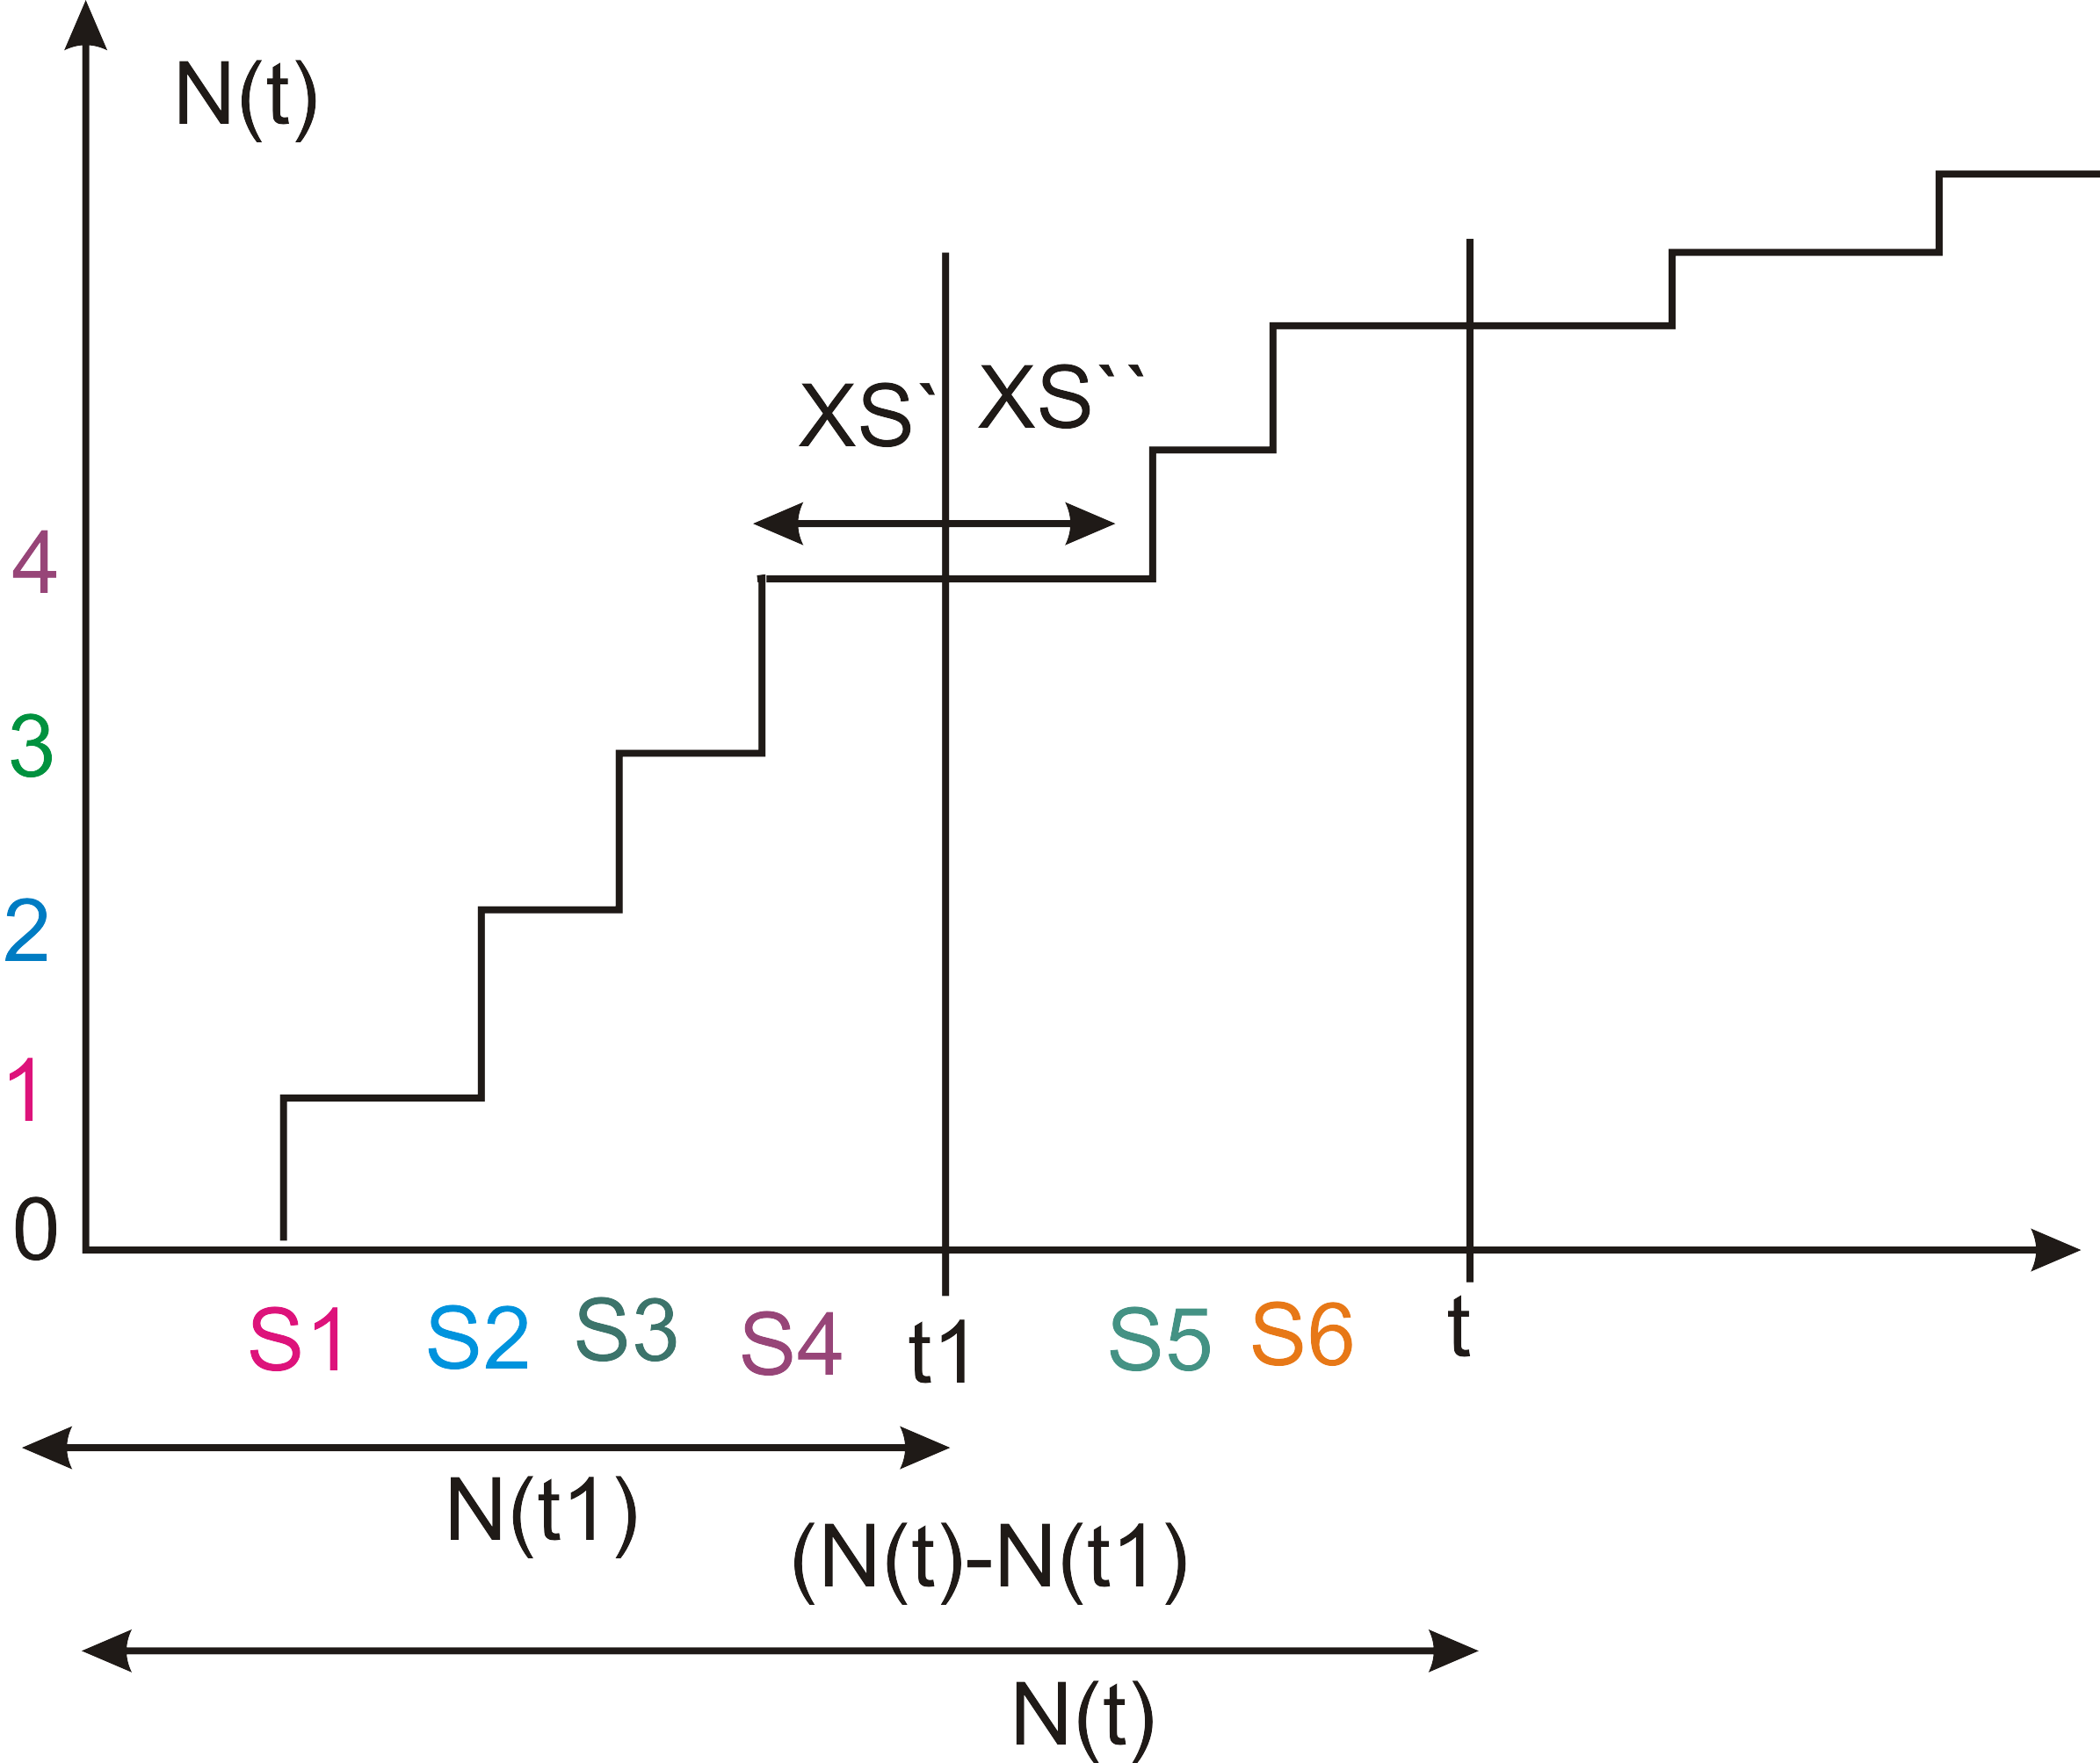
\includegraphics[width=5in, height=2.3in]{Figures/notes2.png}\\
 % \caption{}\label{}
\end{figure}
\begin{eqnarray*}
% \nonumber to remove numbering (before each equation)
  N_t-N_{t_{1}} &=& 2 \\
  N_t-N_{t_{1}} &\perp& N_t  ~(\text{independent}~ \text{increment property})
\end{eqnarray*}
\begin{eqnarray*}
% \nonumber to remove numbering (before each equation)
  X_{5}^{'}+ X_{5}^{''}&=& X_{5} \sim exp(\lambda). \\
  P (X_{5}>X_{5}^{'} &|& X_{5}>X_{5}) \\
   &=&  P (X_{5} > x) \\
   N_t-N_{t_{1}} &\perp& N_{t_{1}}. 
\end{eqnarray*}
Independent increment hold only if inter arrival time is exponential. Thus, we show the independence of $(N_{t_{n}}-N_{t_{n-1}},...,N_{t_{1}})$. Now, the inter arrival times are $iid$ and exponentially distributed gives the result  $N_{t_{2}}-N_{t_{1}} \sim N_{t_{2}-t_{1}}$. 
\subsection{Various Characterizations of the Poisson Process}

\noindent In the previous section, we have shown that Poisson process has stationary, independent increment property. Now, consider any point process with independent, stationary increments. From the discussion in the previous section, it follows that the inter arrival times has to be $iid$ with exponential distribution. Such a characterization does not exclude the possibility of more than one arrival at any time instant. So, if in addition we impose that the jump size should be unity along with stationary, independent increments, the process will be a Poisson process. There are stochastic processes which are stationary, independent increment and not Poisson Process. For eg., batch/ compound Poisson point process, Brownmans motion.
\begin{defn}
\end{defn}
 A point process $\{N_t,~t\geq 0\}$ is said to be Poisson process with rate $\lambda$ if it has stationary, independent property and $P (N_{t}=n)= \frac{(\lambda t)^{n}}{n!} e^{-\lambda t}, n=0,1,2,....$\\

We can have another yet another characterization of the Poisson process.

\begin{figure}[h!]
\center
  % Requires \usepackage{graphicx}
  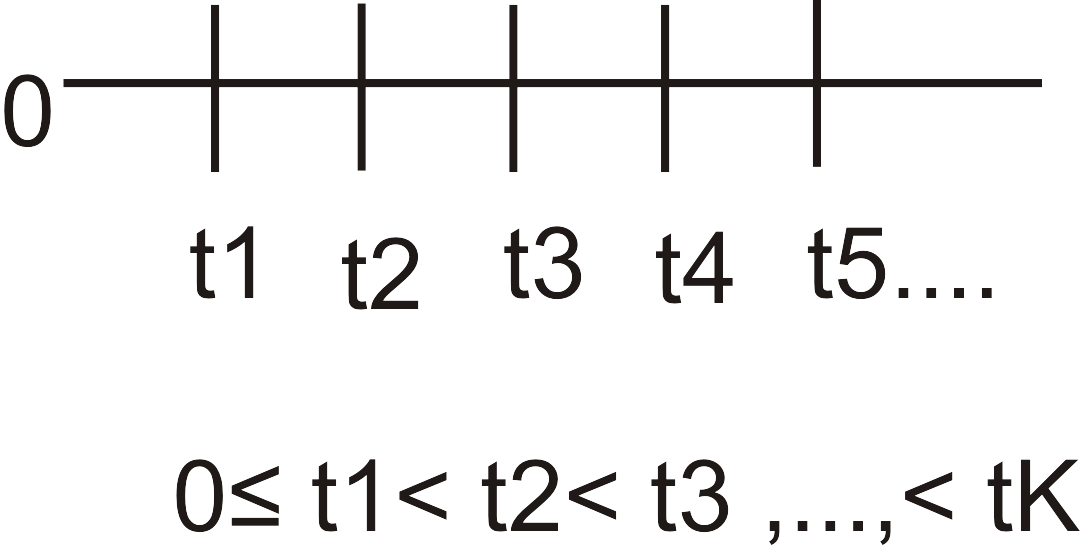
\includegraphics[width=2.8in, height=0.9in]{Figures/SPQT.png}\\
 % \caption{}\label{}
\end{figure}
\noindent Consider a stationary, independent increment point process $\{N_t,~t\geq 0\}$. And  \\
\begin{eqnarray*}
% \nonumber to remove numbering (before each equation)
  P[N_{t_{1}}= n_{1},N_{t_{2}}-N_{t_{1}}= n_{2},..., N_{t_{k}}-N_{t_{k-1}} =n_{k}] \\
   &=& \frac{(\lambda t_1)^{n_{1}}}{n_1!} e^{-\lambda t_{1}} \frac{(\lambda(t_{2}-t_{1}))^{n_{2}}}{n_{2}!} e^{-\lambda (t_{2}-t_{1})} \hdots\\
   & \frac{(\lambda(t_{k}-t_{k-1}))^{n_k}}{n_{k}!} e^{-\lambda (t_{k}-t_{k-1})}.
\end{eqnarray*}
\noindent It will also characterize Poisson Process. Stationary, independent increment property and\\
\begin{eqnarray*}\label{eqn1}
P[N_{t}=0] &=& 1-\lambda t + o(t) \\
  P[N_{t}=1] &=& \lambda t + o(t) \\
  P[N_{t}>1] &=& o(t)
\end{eqnarray*}
We first show that Poisson process satisfy the above set of equations. We have shown that the Poisson process has stationary, independent increment property  and 
\begin{eqnarray*}
% \nonumber to remove numbering (before each equation)
  P[N_t= n] &=&  e^{-\lambda t} \frac{(\lambda t)^{n}}{n!}, n=0,1,2,...
  \end{eqnarray*}
  \begin{eqnarray*}
  P[N_{t}=0] &=& e^{-\lambda t} = 1-\lambda t + o(t).\\
   P[N_{t}=1]&=& e^-\lambda t (\lambda t) \\
  &=& e^-\lambda t^{(1-e^-\lambda t+ o(t))}\\
   &=& \lambda t- \lambda^{2} t^{2}+ o(t) \lambda t.
   \end{eqnarray*}
   Since $\frac{\lambda^{2} t^{2}}{t} =  \lambda^{2} t$ and $\lim _{t\downarrow 0}\lambda^{2} t= 0$, $\lambda^{2} t^{2} =o(t)$. Consider  $\lambda t o(t) = 0$.   $\lim _{t\downarrow 0}\frac{\lambda t o(t)}{t} = \lambda \lim _{t\downarrow 0} o(t)$. Since sum of two $o(t)$ terms is again an $o(t)$ term, $P[N_{t}=1]= \lambda t + o(t)$. Since the three probability terms given should sum up to 1, $ P[N_{t}>1]=o(t)$. So, we showed that the  Poisson Process has the above stated property. Now, we show the converse. We will show that $X_{1}\sim exp (\lambda )$. We would like to show that\\
\begin{eqnarray*}
% \nonumber to remove numbering (before each equation)
  P[X_{1}>t] &=&  e^-\lambda t, t\geq 0\\
  Let f(t) &=& P[X_{1}>t],~ t\geq 0 \\
  s>0, f(t+s) &=&   P[X_{1}>t+s]\\
   &=& P[N_{t}=0, N_{t+s}-N_{t}=0]  \\
   &=& P[N_{t}=0] P[N_{t+s}-N_{t}=0|N_{t}=0 ] \\
   &\stackrel{(a)}{=}& P[N_{t}=0] P[ N_{t+s}-N_{t}=0]\\
   &\stackrel{(b)}{=}&  P[X_{1}>t] P[N_{s}=0]  \\
   &=& P[X_{1}>t] P[X_{1}>s] \\
   &=& f(t) P(N_{s}=0) \\
   &=& [1- \lambda s + o(s)] f(t) \\
  f(t+s) &=& P [1- \lambda s + o(s)] f(t)\\
  \frac{f(t+s)-f(t)}{s} &=& \frac{o(s)}{s}f(t)- \lambda f(t) \\
  \lim_{s\downarrow0}  \frac{f(t+s)-f(t)}{s}  &=& f(t) \times 0 - \lambda f(t) = -\lambda f(t) \\
 f'(t) &=& - \lambda f(t), t\geq 0.
\end{eqnarray*}
where (a) follows from independent increment property and (b) follows from stationary increment property.We have shown that $f$ has a derivative and is equal to $-\lambda f(t)$.\\
\begin{eqnarray*}
% \nonumber to remove numbering (before each equation)
   P[N_{t}=0] &=& 1- \lambda (t)+ 0(t) \\
  \lim _{t\downarrow0}P[N_{t}=0] &=& 1 \\
  1= \lim _{t\downarrow0}P[N_{t}=0]&=& \lim _{t\downarrow0}P[X_{1}>t] \\
   &=& P[X_{1}>0]  \\
  \therefore f(0) &=& 1
  \end{eqnarray*}
  Solve $\frac{df(t)}{dt} = -\lambda f(t), ~t\geq 0$, $f(0)= 1$. We get $f(t) = e^{-\lambda t}$.
   \begin{eqnarray*}
  \therefore f(t) &=&  P[X_{1}>t]= e^{-\lambda t}.\\
  X_{1}&\sim & exp (\lambda ).
\end{eqnarray*}
To show that $X_{1}, X_{2}$ both are independent\\
\begin{eqnarray*}
% \nonumber to remove numbering (before each equation)
 P(X_{1}=t_{1}, X_{2}=t_{2}) && t_{1} >0, t_{2}>0\\
  P(X_{1}=t_{1})P (X_{2}=t_{2}| X_{1}=t_{1})&=& \lambda e^{-\lambda t_{1}} \\
   &=& \lambda e^{-\lambda t_{1}} P[N_{t_{1}+t_{2}}-\delta=1,N_{t_{1}+t_{2}}=2|N_{t_{1}}=1) \\
   &=& \lambda e^{-\lambda t_{1}} p[Nt_{2}=1] \\
   &=& \lambda e^{-\lambda t_{1}} \lambda e^{-\lambda t_{2}}  \\
   X_{1} \perp X_{2}&and & X_{1}, X_{2} \sim exp (\lambda).
\end{eqnarray*}
Thus completing the proof. 

We study these characterizations because Poisson process is a fundamental process (just like Gaussian process among the class of distributions).

\subsection{Non-Homogeneous Poisson Process}
 From the characterization of Poisson process just stated, we can generalize to non-homogeneous Poisson process. The rate of Poisson process $\lambda$, in practical case, keeps changing. It is not clear, how to generalize the definition of Poisson process to the non-homogeneous case (where $\lambda$ is not fixed) from the first two characterizations. $m(t)$ is the rate at time $t$. Let $\bar{m}=\int_{0}^{t}m(s)ds$. 
 \begin{eqnarray*}
 P[N_{t}=0]&=&1-m(t)+o(t). \\
  P[N_{t+\triangle}-N_t=0] &=& =1-m(t)\triangle+o(\triangle). \\
   P[N_{t+\triangle}-N_t=1] &=& = m(t)\triangle+o(\triangle). \\
   P[N_{t+\triangle}-N_t>1] &=& =  o(\triangle). \\
   \end{eqnarray*}
 We will show that the distribution of $N_t$ for each $t$ is given by
 \begin{eqnarray*}
 P(N_t=n)=\frac{(\bar{m}(t))^n}{n!}e^{-\bar{m}(t)}.
 \end{eqnarray*}
\begin{eqnarray*}
% \nonumber to remove numbering (before each equation)
  f(t) &=& P[N_{t}=0] \\
  f(t+\triangle) &=& P[N_{t+\triangle}=0] \\
   &=&  P[N_{t}=0, N_{t+\triangle}-N_{t}=0]\\
   &\stackrel{(a)}{=}& P[N_{t}=0] P[N_{t+\triangle}-N_{t}=0]\\
   &=& f(t)[1-m(t)\triangle +o(\triangle)].\\
\frac{f(t+\triangle)-f(t)}{\triangle} &=& -m(t) f(t) +f(t) \frac{0(\triangle)}{\triangle}. \\
  \lim_{\triangle\downarrow 0}\frac{f(t+\triangle)-f(t)}{\triangle} &=& -m(t) f(t) \\
 \frac{d f(t)}{t} &=& -m(t) f(t),  \\
 \end{eqnarray*}
 where (a) follows from independent increment property. Since, $\overline{m}(t)=\int ^{t}_{0} m(s) ds $, $f(t)=P[N_{t}=0]$, $ f(0)=P[N_{0}=0] =1$ the solution of the differential equation can be verified to be $f(t)=e^{-\overline{m}(t)}$, as follows: 
 \begin{eqnarray*}
     f(0)&=& e^{-\overline{m}(t)}\\
  &=& e^{-0}=1 \\
  f'(t) &=& e^{-\overline{m}(t)}\frac{d}{dt} \int^{t}_{0}m(S) ds\\
  &=& m(t)e^{-\overline{m}(t)}, t\geqslant 0 \\
  \end{eqnarray*}
  
  \begin{eqnarray*}
  P[N_{t+\triangle}-N_{t}=0] &=& 1-m(t)\triangle +o(\triangle) \\
  P[N_{\triangle}-N_{0}=0] &=& 1-m(0)\triangle +o(\triangle) 
  \end{eqnarray*}
  Since $ N_{0}=0$, 
  \begin{eqnarray*}
   P[N_{\triangle} =0]&=& 1-m(0)\triangle +0(\triangle) \\
  \lim_{\triangle\downarrow 0}f(\triangle) &=& f(0)=1.
\end{eqnarray*}
We have shown $P[N_{t}=0] = e^{-\overline{m}(t)}$. Similarly, for any $n$, we can show the result.

\subsection{Conditional Distribution of the Arrival Instants}
\noindent For the Poisson process $\{N_{t}, t\geq 0\}$ with rate $0<\lambda< \infty$, we would like to find the density.
\begin{eqnarray*}
% \nonumber to remove numbering (before each equation)
  P(S_{1}\mid N_{t}=1), t>0 \\
  P_{S_1}(S \mid N_{t}=1) \\
  P(s\leq S_{1} \leq s+h \mid N_{t}=1)\\
   &\approx& h P_{S_1}(S \mid N_{t}=1 \\
  P(s\leq S_{1}< s+h \mid N_{t}=1)\\
   &=& \frac{P(s\leq S_{1}< s+h,N_{t}=1)}{P(N_{t}=1)}\\
   &=& \frac{P[s\leq S_{1}<s+h,X_{2}>t-(s+h))}{\lambda t e^{-\lambda t}} \\
   &=& \frac{h \lambda e^{-\lambda h} e^{-\lambda (t-(s+h))}}{h{\lambda t} e^{-\lambda t}}.
   \end{eqnarray*}
   Take  $\lim _{h\rightarrow 0}\frac{1}{t}{e^{-\lambda h}} =\frac{1}{t}.$ Thus, the conditional density is the density of a uniform random variable distributed over the interval $[0,t].$ This property of Poisson process can be generalized. For $0<s_{1}<s_{2},.., s_{n}<t$ and $n=1,2 \hdots$ \\

\begin{eqnarray*}
% \nonumber to remove numbering (before each equation)
    &P[s_{1}\leq S_{1}<s_{1}+h, s_{2}\leq S_{2}<s_{2}+h, ...s_{n}\leq S_{n}\leq s_{n}+h \mid N_{t}=n]  \\
   &=   \frac{P[s_{1}\leq S_{1}<s_{1}+h, s_{2}\leq S_{2}<s_{2}+h,...,s_{n}\leq S_{n}\leq s_{n}+h,N_{t}=n]}{P[N_{t}=n]} \\
   &=  \frac{P[s_{1} \leq S_{1}<s_{1}+h_{1},s_{2}-s_{1}\leq X_{2}<s_{2}- (s_{1}+h),..., X_{n+1}> t-s_{n}]}{P[N_{t}=n]} \\
   &\stackrel{(a)}{=}  \frac{P[s_{1 \leq S_{1}<s_{1}+h}]P[s_{2}-s_{1}\leq X_{2}<s_{2}-s_{1}+h] P[X_{n+1}>t -s_{n}]}{P[N_{t}=n]}\\
   &=  \frac{\lambda h e^{-s_{1}\lambda}h \lambda e^{-(s_{2}-s_{1})\lambda},..., e^{-(t-s_{n})\lambda}}{(\lambda t)^{n}\frac{e^{-\lambda t}}{n!}} 
   \end{eqnarray*}
   \begin{eqnarray*}
    \lim _{h\rightarrow 0} \frac{ \lambda h e^{-s_{1}\lambda}h \lambda e^{-(s_{2}-s_{1})\lambda},... e^{-(t-s_{n})\lambda}}{h^{n}(\lambda t)^{n}\frac{e^{-\lambda t}}{n!}}=\frac{n!}{t^{n}}.
\end{eqnarray*}
where (a) follows as $X_i$s are independent. Thus, if $U_{1},... U_{n}$ are $iid$ Uniform random variables in $[0,t]$, conditioned on $\{N_t=n\}$, the $n$ arrival instants have the same distribution as the order statistics  of $U_1 \hdots U_n$.\\
We give some more properties of the Poisson process. \\
Suppose, ${N_{1 }(t), t \geq  0}$ Poisson process unit rate $\lambda _{1}$, ${N_{2} (t), t \geq  0}$ Poisson process unit rate $\lambda _{2}$. Further, assume that the two Poisson processes are independent of each other. Let $N(t)= N_{1}(t) +N_{2}(t)$. \\

\textbf{Claim}: ${N(t), t \geq  0}$ is a Poisson process with rate $\lambda_{1}+\lambda_{2}$.\\ 
\textbf{Proof}: Need to show that
\begin{eqnarray*}
% \nonumber to remove numbering (before each equation)
 \frac{P[Nt=n]  [(\lambda_{1}+\lambda_{2}t]^{n}e^{-\lambda_{1}+\lambda_{2}t}}{n!}\\
\end{eqnarray*}
and $\{N_t\}$ has stationary, independent increments.\\
For $N_{1}(t)$,  arrivals in $(t_{1}, t_{2})\perp (t_3,t_{4})$. Similarly, for $N_{2}(t)$ arrivals in $(t_{1}, t_{2})\perp (t3,t_{4})$. Therefore, $N(t)$ has independent increment property. Similarly, we can argue out stationary increment property of $\{N_t\}$.\\
\begin{eqnarray*}
% \nonumber to remove numbering (before each equation)
  P[N(t)=n] &=& P[N_{1}(t)+ N_{2}(t)= n] \\
   &=& \sum_{n1} P [N_{1}(t)=n_{1},N_{2}(t)= n-n_{1} ] \\
  &=& \sum_{n_{1}}\frac{e^{-\lambda _{1}t}(\lambda_{1}t)^{n_{1}}}{n_{1}!}e^{-\lambda_{2}t}\frac{(\lambda_{2}t)^{(n-n_{1})}}{(n-n_{1})!} \\
   &=&\sum_{n_{1} (\lambda _{2}t)} \frac{e^{-(\lambda_{1}+\lambda_{2})t} (\lambda_{1}t)^{n1}(\lambda_{2}t)^{-n_{1}}}{n_{1}! (n-n_{1})!} \\
   &=& \frac{e^{-(\lambda_{1}+\lambda_{2})t}}{n!}\sum^{n}_{n_{1=0}}\left(\frac{\lambda_{1}}{\lambda_{2}}\right)^{n_{1}}\left(\frac{\lambda_{2}}{n_{1}!}\right)^{n}\frac{n!}{(n-n_{1})!} \\
   &=&  \frac{e^{-(\lambda_{1}+\lambda_{2})t}}{n!}(\lambda_{1}+\lambda_{2})^{n}t^{n}
\end{eqnarray*}
\begin{figure}
\centering
  % Requires \usepackage{graphicx}
  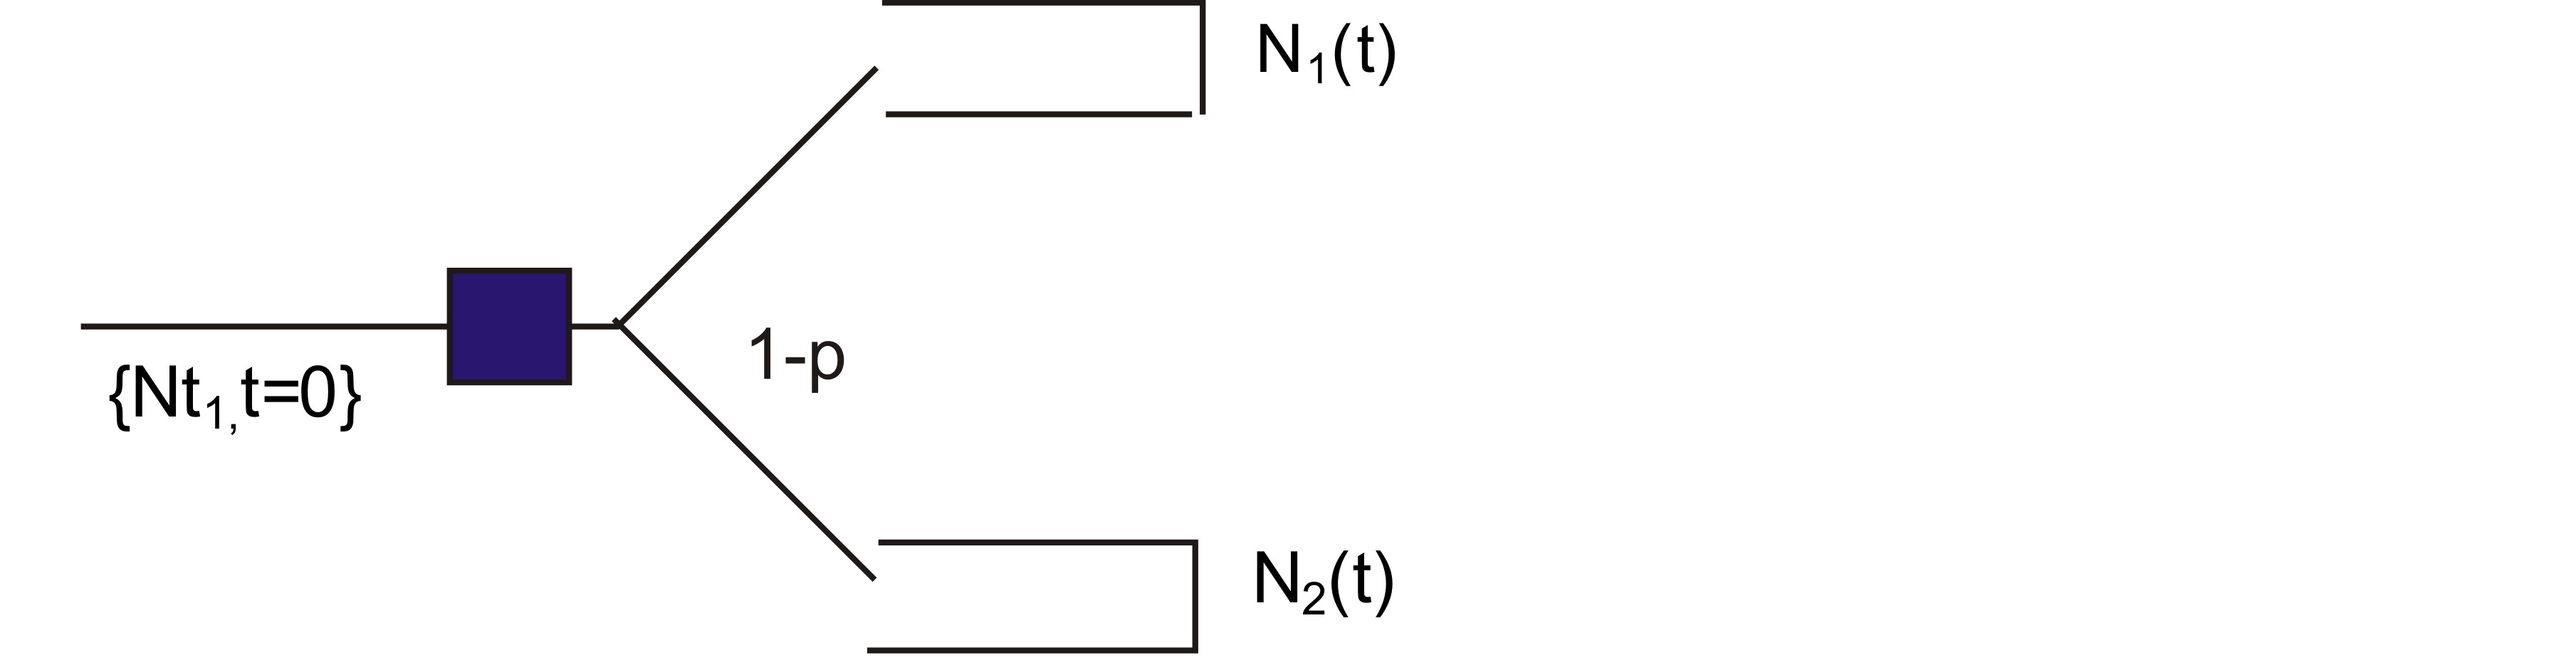
\includegraphics[width=5.0in]{Figures/comment.PNG}\\
 % \caption{}\label{}
\end{figure}

\textbf{Comment}: If independence condition is removed, the statement is not true.\\

\textbf{Claim}:${N_{1}(t), t\geq 0}, {N_{2}(t), t \geq 0}$ are Poisson processes with rates $\lambda p$ and $\lambda (1-p)$ and these process are independent of each other.  

\textbf{Proof:} To show that ${N_{1}(t), t \geq 0}$ is a Poisson process with rate $\lambda p$, we show that it is stationary independent increment process with the distribution
\begin{eqnarray*}
% \nonumber to remove numbering (before each equation)
 P[N_{1}(t)= n]  = \frac{(p \lambda t)^{n}}{n!}e^{-\lambda p t}.
\end{eqnarray*}
\begin{figure}
\center
  % Requires \usepackage{graphicx}
  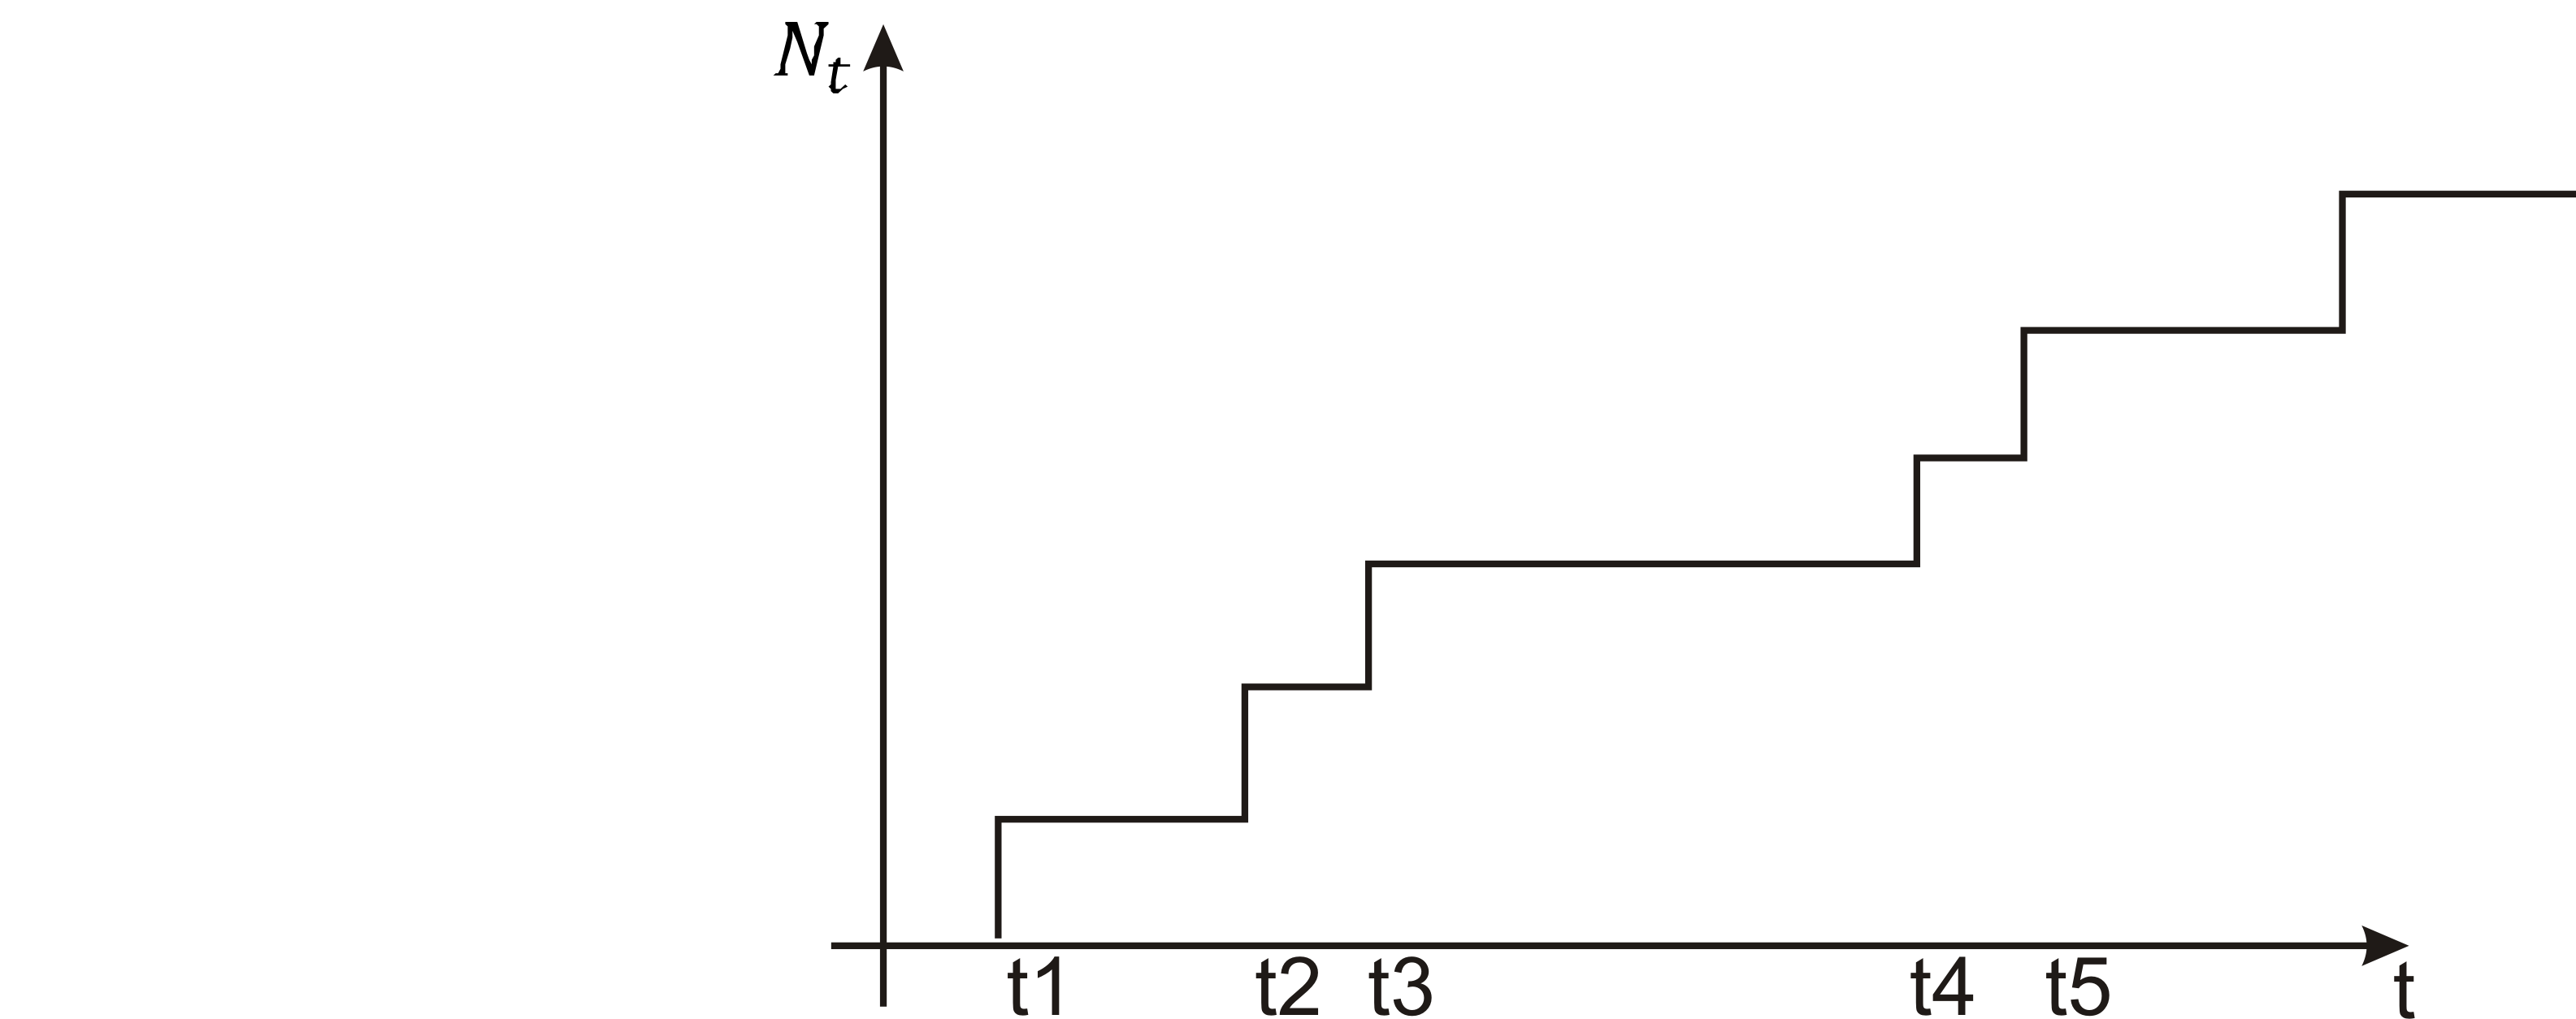
\includegraphics[width=4.5in]{Figures/distr.PNG}\\
 % \caption{}\label{}
\end{figure}
The stationary, independent increment property of the probabilistically filtered processes $\{N_1(t)\}$ and $\{N_2(t)\}$ can be understood and argued out from the example given in the figure. \\
  \begin{eqnarray*}
  % \nonumber to remove numbering (before each equation)
    P[N_{1}(t) =n]&=& \sum^{\infty}_{m=0}P[N(t)=m, N_{1}(t) = n]  \\
   &=& \sum^{\infty}_{m=n}P[N(t)=m] p^{n}(i-p)^{m-n}mC_n\\
   &=&  \sum^{\infty}_{m=n}\frac{e^{-\lambda t(\lambda t)^{m}}}{m!}p^{n}(1-p)^{m-n}(mC_n)\\
     &=& e^{-\lambda t}p^{n}\sum_{m=n}\frac{(\lambda t)^{m-n}}{m!}\frac{(1-p)^{m-n}m!}{n!(m-n)!} \\
     &=& \frac{e^{-\lambda t p}(p \lambda t)^{n}}{n!} \sum^{\infty}_{m=n}e^{-\lambda (1-p)t}\frac{(\lambda (1-p)t)^{m-n}}{(m-n)!} \\
     &=&  \frac{e^{-\lambda t p}(p \lambda t)^{n}}{n!} \sum^{\infty}_{k=0}e^{-\lambda (1-p)t}\frac{(\lambda (1-p)t)^{k}}{k!}  \\
     &=& \frac{e^{-\lambda p t}(p \lambda t)^{n}}{n!}.
  \end{eqnarray*}
To show that 
\begin{eqnarray*}
% \nonumber to remove numbering (before each equation)
   \{N_{1}(t), t \geq 0\}&\perp&\{N_{2}(t), t \geq 0\}  \\
   P[N_{1}(t)&=&n_{1}, N_{2}(t) = n_{2}]\\
    P[N(t) = n_{1}+ n_{2}]&=& \frac{e^{-\lambda t} (\lambda t)^{n_{1}+n_{2}}}{(n_{1}+n_{2})!} \\
   &=&  \frac{e^{-\lambda p t}e^{-\lambda (1-p)t}}{(n_{1}+n_{2})!} -(\lambda t)^{n_{1}+n_{2}}\\
   &=&  \frac{e^{-\lambda p t}e^{-\lambda (1-p)t} (\lambda t)^{n_{1}}(\lambda t)^{n_{2}}}{n_{1}! n_{2}!}
\end{eqnarray*}
In general, we need to show fdds factorize. For measurable $A_1, hdots A_n$, $B_1, \hdots B_m$ and \\
\begin{eqnarray*}
% \nonumber to remove numbering (before each equation)
   0 \leq t_{1}< t_{2}&...&<t_{n}  \\
   0\leq s_{1}<s_{2}&...&s_{m}.
   \end{eqnarray*}
   \begin{eqnarray*}
   P[N_{1}(t_{1})\in A_{1}, N _{2}(t_{2})\in A_{2},\hdots N_{2(s_{1})}\in B_{1}, N_{2}(s_{2})\in B_{2} ..] \\
   =P[(N_{1}(t_{1})\in A_{1}&...&N_{1}(t_{n})\in A_{n})],\\
   P[(N_{2}(S_{1})\in B_{1}&...&N_{2}(S_{m})\in B_{m})].
\end{eqnarray*}

\subsection{Compound (Batch) Poisson Process}
$S_{n}$ = time of arrival of $n^{th}$ batch of customers/ packets.\\
$Z_{n}$ = Size of $n^{th}$ batch.\\
$\{Z_{n}\} iid \perp \{X_{n}\}$.\\
Also, assume stationary, independent increment property.\\
\begin{eqnarray*}
% \nonumber to remove numbering (before each equation)
  N_{t} &=& \sup \{n: S_{n}\leq t \}  \\
  \end{eqnarray*}
   $\overline{N_{t}}$= No of arrivals till time $n$  \\
   \begin{eqnarray*}
   \overline{N_{t}}&=& \sum ^{N_{t}}_{k=0}Z_{k}  ~(\text{No. of arrivals till time $n$}).\\
   \mathbb{E}[\overline{N_{t}}]&=&\mathbb{E}\left[\sum ^{N_{t}}_{k=0}Z_{k}\right]  \\
   &=& \sum^{\infty}_{n=0}\mathbb{E}\left[\sum ^{N_{t}}_{k=0}Z_{k}|N_{t}-n \right] P[N_{t}=n]\\
   &=& \sum^{\infty}_{n=0}P[N_{t}=n]\mathbb{E}\left[\sum^{\infty}_{k=0}Z_{k}|N_{t}=n   \right] \\
   &=& \sum^{\infty}_{n=0} \frac{e^{-\lambda t} (\lambda t)^{n}}{n!} n \mathbb{E}[Z_{1}] \\
   &=& \mathbb{E} [Z_{1}]\mathbb{E} [N_{t}].
   \end{eqnarray*}
   For  $  \alpha>0 $,  \\
   \begin{eqnarray*}
   &\mathbb{E}[e^{\alpha \overline{N_{t}}}]=\mathbb{E}\left[e^{\alpha\sum ^{N_{t}}_{k=0}Z_{k}}\right] \\
   &=& \sum^{\infty}_{n=0}\mathbb{E}\left[ e^{\alpha\sum ^{N_{t}}_{k=0}Z_{k}}| N_{t}=n\right] P[N_{t}=n]\\
   &=&  \sum^{\infty}_{n=0}\mathbb{E}\left[e^{\alpha\sum ^{n}_{k=0}Z_{k}}\right] P[N_{t}=n]\\
   &=&\mathbb{E}[\mathbb{E}[e^{\alpha Z_{1}}]^{N_{t}}]\\
  \mathbb{E} [\beta^{N_{t}}] &=&\sum^{\infty}_{n=0}\frac{(\lambda t)^{n}e^{-\lambda t}}{n!}\beta^{n}\\
   &=&\sum^{\infty}_{n=0}\frac{(\lambda \beta t)^{n}e^{-\lambda \beta t}}{n!}\lambda (\beta t-t)\\
   &=& e^{\lambda t (\beta-t)}
   \end{eqnarray*}
   \textbf{Example:}\\
\begin{figure}[h!]
\center
  % Requires \usepackage{graphicx}
  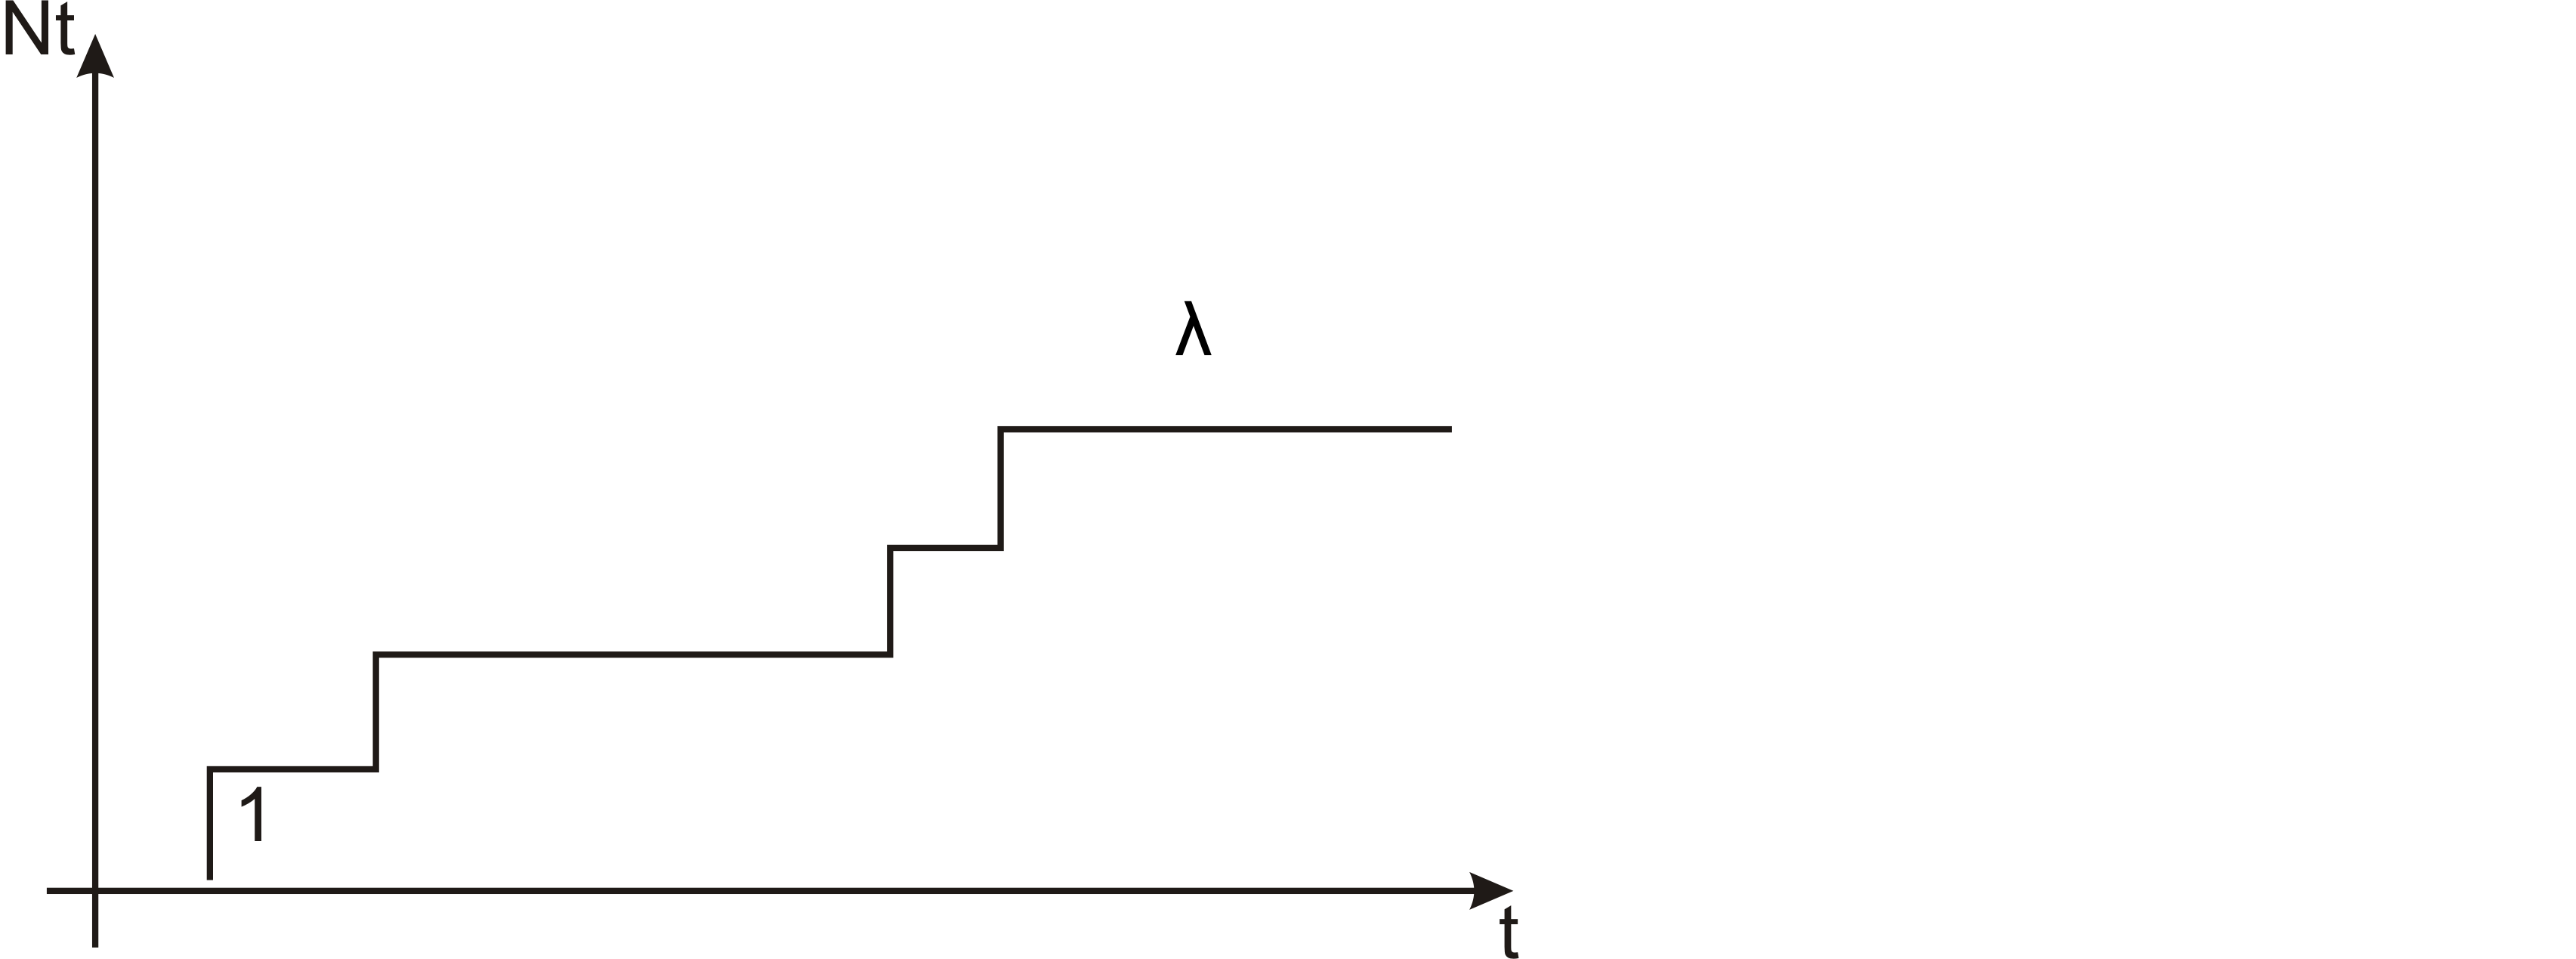
\includegraphics[width=4.5in]{Figures/rate.PNG}\\
 % \caption{}\label{}
\end{figure}
Suppose $\{N_{t}, t \geq 0\}$ Poisson process with rate $\lambda$. 

$\tilde{N_{t}}(w)= N_{t}(w)+f(t+X_{1}(w))$ where $f(t)$=0, if $t$ is irrational and $f(t)$=t, if $t$ is rational.\\
\begin{eqnarray*}
% \nonumber to remove numbering (before each equation)
  P[\tilde{N_{t}}\neq N_{t}] &= P[\omega:t+X_{1}(\omega) \text{is rational}],\\
  &= P[\omega:X_1(\omega)  \text{is rational} ] =0.
\end{eqnarray*}
 
\begin{eqnarray*}
% \nonumber to remove numbering (before each equation)
  P[\tilde{N_{t}}= N_{t}] &=& 1\\
  P[\tilde{N_{t_1}}= N_{t_1},\tilde{N_{t_2}}= N_{t_2} ] \\
  &=& \sum_{n_{1},n_{2}}P[\tilde{N_{t1}}= N_{t_1},\tilde{N_{t_2}}= N_{t_2}, N_{t_1}=n_1, N_{t_2}=n_2 ] \\
   &=& 1
\end{eqnarray*}
$\{\tilde{N_{t}}\}, \{N_{t}\}$ have same fdds.\\
$\{\tilde{N_{t}}(\omega)\}$ can take non-integer values and is not non-decreasing.\\
Two process can have same distribution but sample path behaviour can be quite different.\\
\end{document}